% pdflatex --shell-escape lecture9.tex & pdflatex --shell-escape lecture9.tex  
% created by Uwe Schadewald
% modified by Mathias Kuntze and Ahmet Uysal
% Add, handout to documentclass arguments for condensed pdf
\documentclass[presentation, 8pt, mathserif, t]{beamer} % , aspectratio=169
\usepackage[english]{babel}
\usepackage{pgf,graphicx}
\usepackage{amsmath, amssymb}
\usepackage[utf8]{inputenc}
\usepackage{lmodern}
\usepackage{palatino}
\usepackage{multimedia}
\usepackage{pgfpages} 
\usepackage{tikz}
\usepackage{datetime}
\pdfoptionpdfminorversion=5

\usepackage{caption}
\usepackage{subcaption}
% if else
\usepackage{ifthen}
% extend table options
\usepackage{tabularx} 
\usepackage{booktabs}
\usepackage{multicol}
\usepackage{multirow}
\usepackage{eso-pic}  % package to set background image
\usepackage[calc]{picture}

% Packages and stuff for ToDo list like itempoints
\usepackage{pifont}
\newcommand{\cmark}{\ding{51}}%
\newcommand{\xmark}{\ding{55}}%
\newcommand{\open}{$\square$}
\newcommand{\done}{\rlap{$\square$}{\raisebox{1pt}{\large\hspace{1.5pt}\cmark}}\hspace{-2.5pt}}
\newcommand{\wontfix}{\rlap{$\square$}{\raisebox{1pt}{\large\hspace{1.5pt}\xmark}}}
\newcommand{\notsure}{\rlap{$\square$}{\raisebox{0.8pt}{\large\hspace{1.5pt}\textbf{?}}}}



% side bar and footer
\setbeamertemplate{headline}{	
	\leavevmode
	\vspace{-4em}	
	\hbox{		
		\begin{beamercolorbox}[wd=0.85\paperwidth,ht=10ex,dp=8ex,center]{}%			
			% navigation with subsections as dots
			\hspace{3.5em}\insertnavigation{0.7\paperwidth}{\hskip0pt plus1fill} % add navigation in footer						
			% navigation with sections, no subsections
			% \insertsectionnavigationhorizontal{0.6\paperwidth}{\hskip0pt plus1fill}{} \\ % add navigation in footer}
			
		\end{beamercolorbox} 				
	}
	\vskip0pt
}


\setbeamertemplate{footline}{	
	\leavevmode
	\vspace{-3em}
	\hbox{
		\begin{beamercolorbox}[wd=.33\paperwidth,ht=2.25ex,dp=1ex,left]{author in head/foot}%
			\hspace{5em}
			\insertshortauthor
		\end{beamercolorbox}
		\begin{beamercolorbox}[wd=.33\paperwidth,ht=2.25ex,dp=1ex,center]{title in head/foot}%
			\insertshorttitle \ - \insertshortsubtitle
		\end{beamercolorbox}	
		\begin{beamercolorbox}[wd=0.30\paperwidth,ht=10ex,dp=8ex,right]{pagenumber in head/foot}			 	
			\insertframenumber % add page numbers
		\end{beamercolorbox}
	}			
	\vskip0pt
}



\setbeamertemplate{frametitle}{
	\ifthenelse{\equal{\insertframesubtitle}{}}{
		\vspace{0.6cm}
		\huge{\insertframetitle}
	}{
		\vspace{0.6cm}
		\small{\insertframetitle}\\
		\vspace{0.3cm}
		\huge{\insertframesubtitle}
    }		
}

	
% enumerate sections
\setbeamertemplate{section in head/foot}{\hfill\insertsectionheadnumber.~\insertsectionhead}
%\setbeamertemplate{section in head/foot shaded}{\color{structure!50}\hfill\insertsectionheadnumber.~\insertsectionhead}
\setbeamertemplate{section in toc}{\inserttocsectionnumber.~\inserttocsection}

%enumerate subsections
\setbeamertemplate{subsection in head/foot}{\hfill\insertsubsectionheadnumber.~\insertsubsectionhead}
\setbeamertemplate{subsection in head/foot shaded}{\color{structure!50}\hfill\insertsubsectionheadnumber.~\insertsubsectionhead}
%\setbeamertemplate{subsection in toc}[subsections numbered]
\setbeamertemplate{subsection in toc}{\vskip0.5em\leftskip=2em\inserttocsubsection\par}

%--------------------------Common------------------------------------------------------
\setbeamercovered{transparent} % make the beamer theme invisible
\usefonttheme{structurebold}
\beamertemplatenavigationsymbolsempty % set navigations helper function to off
\setbeamertemplate{bibliography item}[text]
\setbeamertemplate{note page}[plain]

%\setlist[itemize,1]{label={$\bullet$}} % \item are using bullets
\setbeamertemplate{itemize items}[circle]
	
	

	
% create a new command to show it on two screens
% I'm using dspdfviewer.
\newcommand{\setDualView} {
	\setbeameroption{show notes on second screen=right}
}

%\AtBeginSection[]{\subsection{}}
\newcommand{\addcite}[1]{%
	\AddToShipoutPictureFG*{%
		\AtPageLowerLeft{%
			\put(0.90\paperwidth,5em){											
				\tiny{
					\cite{#1} 
				}			
			}
		}
	}	
}

% insert a frame with references -> use bibtex
\newcommand{\insertReferenceFrame}[3]{%
	\section{#1}
	\begin{frame}[allowframebreaks]
		\frametitle{#1}
		\bibliographystyle{#2}
		\bibliography{#3}
	\end{frame}	
}

\AtBeginSection[]{\subsection{}}
	





\usepackage{../KU-Beamer-Template/style/koc} 
\usepackage{minted}
\usepackage{upquote}
\usepackage{graphicx}

\title{KOLT Python}
\subtitle{Third-Party Packages} 
\newdate{date}{25}{11}{2019}
\date{\displaydate{date}}
\author{Ahmet Uysal}

\titlegraphic{
\includegraphics[scale=0.2]{../KU-Beamer-Template/style/images/logo_kolt.pdf}}

\setbeamercovered{invisible} % transparent

\begin{document}
    \maketitle

    \frame{\frametitle{Agenda}\tableofcontents}


    \section{Installations}
    \begin{frame}{Installing Python}
        \LARGE
        \begin{itemize}
            \item Go to \href{https://www.python.org/downloads/}{\underline{\textit{python.org/downloads}}}
            \pause
            \item Install the latest version of Python for your operating system
            \pause
            \item (Windows only) Make sure to add python to the \texttt{environment variables} by checking the corresponding permission on the installation or by hand
            \pause
            \item Check the installation by running \textbf{\texttt{python}}(Windows)/\textbf{\texttt{python3}}(macOS/Linux) in terminal.
        \end{itemize}
        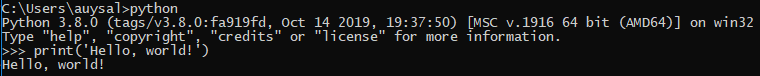
\includegraphics[width=\textwidth]{images/cmd_helloworld.PNG}
    \end{frame}
     
    \begin{frame}[t]{Installing an Editor/IDE(Integrated Development Environment)}
        \vspace{-4mm}
        \begin{columns}[t] 
            \begin{column}[t]{0.66\linewidth}
                \LARGE
                \begin{itemize}
                    \item Having a specialized editor/IDE can help a lot. 
                    \item We will use Visual Studio Code but you are free to use any editor/IDE of your choice.
                    \item Get Visual Studio Code from \href{https://code.visualstudio.com/download}{\underline{\textit{code.visualstudio.com/download}}}
                \end{itemize}
            \end{column}
            
            \begin{column}{0.33\linewidth}
                \begin{center}
                    
\includegraphics[width=0.8\linewidth]{images/vscode_icon.png}						
                \end{center}
            \end{column}
        \end{columns}
     \end{frame}

     \begin{frame}{Configuring Visual Studio Code for Python}
        \LARGE
        \begin{itemize}
            \item Install Python extension for VS Code.
            \pause
            \item Select the Python(3.8.0) Interpreter in VS Code.
            \pause
            \item For more information, visit \href{https://code.visualstudio.com/docs/python/python-tutorial}{\underline{\textit{VS Code Python Tutorial}}}.
        \end{itemize}
        \centering
        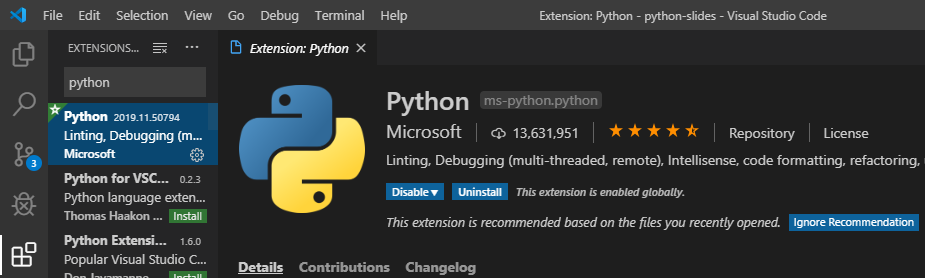
\includegraphics[width=0.75\linewidth]{images/python_extension.PNG}						
     \end{frame}

    \section{Package Management}

    \begin{frame}
        \frametitle{Python Package Index (PyPI)}
        \pause
        \huge
        Repository of software for the Python programming language.
        \pause
        \begin{itemize}
            \item 23,000+ Python3 packages.
            \pause
            \item If you want a package, PyPI probably has it. 
        \end{itemize}
        \pause
        Visit \href{https://pypi.org/}{\underline{\textit{pypi.org}}} to explore packages.
    \end{frame}

    \begin{frame}
        \frametitle{pip}
        \LARGE
        \pause
        \begin{itemize}
        \item Recommended tool for installing Python packages.
        \pause
        \item \textbf{\texttt{pip}} is already installed with modern Python distributions.
        \pause
        \item Try \texttt{pip -V} on your command line/terminal(\texttt{pip3 -V} for Macs). 
        \end{itemize}
        \pause
        \texttt{\$ pip -V}\\
        \texttt{pip 19.2.3 from --PATH\_TO\_PIP-- (python 3.8)}\\
        \pause
        \begin{center}
            \huge
            \textbf{Any problems?}            
        \end{center}
        
    \end{frame}

    \begin{frame}
        \frametitle{Common pip commands}
        \LARGE
        \pause
        \textbf{Install a package:}\\
        \pause
        \texttt{\$ pip \textbf{install} package\_name}  \# latest version \\
        \pause
        \texttt{\$ pip \textbf{install} package\_name==1.0.1}  \# specific version \\
        \pause
        \texttt{\$ pip \textbf{install} package\_name>=1.0.1}  \# minimum version \\
        \pause        
        \textbf{Uninstall a package:}\\
        \pause        
        \texttt{\$ pip \textbf{uninstall} package\_name}\\
        \pause
        \textbf{Update a package:}\\
        \pause
        \texttt{\$ pip \textbf{install --upgrade} package\_name}\\
        \pause
        \textbf{Search PyPI for matches:}\\
        \pause
        \texttt{\$ pip \textbf{search} query}
    \end{frame}

    \section{Virtual Environments}

    \begin{frame}{Virtual Environments}
    
    
    \end{frame}

    \begin{frame}{}
        
    
    \end{frame}

    \section{Example: Telegram Bot}
    
    \begin{frame}{}
    
        
    
    \end{frame}

    \begin{frame}{}
    
        
    \end{frame}
    
\end{document}